\documentclass[a4paper]{sbgames}               % final
%\usepackage[scaled=.92]{helvet}
\usepackage{times}
\usepackage{graphicx}

%% use this for zero \parindent and non-zero \parskip, intelligently.
\usepackage{parskip}

%% the 'caption' package provides a nicer-looking replacement
\usepackage[labelfont=bf,textfont=it]{caption}

\usepackage{listings}
\usepackage{color}

\definecolor{dkgreen}{rgb}{0,0.6,0}
\definecolor{gray}{rgb}{0.5,0.5,0.5}
\definecolor{mauve}{rgb}{0.58,0,0.82}

\lstset{frame=tb,
  language=C,
  aboveskip=3mm,
  belowskip=3mm,
  showstringspaces=false,
  columns=flexible,
  basicstyle={\small\ttfamily},
  numbers=none,
  numberstyle=\tiny\color{gray},
  keywordstyle=\color{blue},
  commentstyle=\color{dkgreen},
  stringstyle=\color{mauve},
  breaklines=true,
  breakatwhitespace=true,
  tabsize=3
}

\usepackage{url}
\usepackage[utf8]{inputenc}
%% Paper title.
\title{Computer Graphics}

%% Author and Affiliation (multiple authors). Use: and between authors

\author{Alexandre Tolstenko Nogueira\\InfiniBrains\\tolstenko@infinibrains.com.br 
%        \and Name2 B. Surname2\\ Name3 C. Surname3\\ ZZZZ University
%        \and Name4 D. Surname4\\ Farwest Research Center 
}
\contactinfo{\{name1,name3\}@xxx.yyyy.yyy \\
             *name2@zzzz.vvvv.vvv
}
%% Keywords that describe your work.
\keywords{Real-time Strategy, Relief Mapping, Shortest Path Algorithm, First Person Shooting}

%% Start of the paper
% Attention: As you need to insert EPS images in Postscript, 
% you need to insert PDF images into PDFs. 
% In the text, extensions cancbe omitted (latex use .eps, pdflatex get .pdf) 
% To convert them: epstopdf myimage.eps
\begin{document}

%\teaser{
%  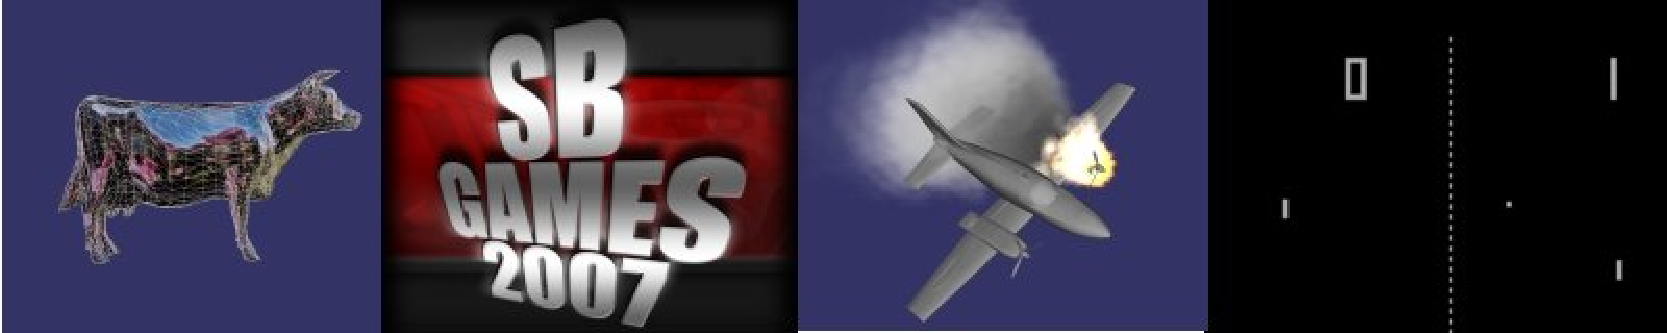
\includegraphics[width=\linewidth]{sample.pdf}
%  \caption{Optional image}
%}

%% The ``\maketitle'' command must be the first command after the
%% ``\begin{document}'' command. It prepares and prints the title block.

\maketitle

%% Abstract section.

%\begin{abstract}
%  This meta-paper describes the model to be used in papers and posters
%  for SBGames. In the subsection Author's contact, make reference to
%  the same symbol used in the affiliation.
%\end{abstract}

%% The ``\keywordlist'' command prints out the keywords.
%\keywordlist
%\contactlist

\section{Atividade Aula 3 - Introdução a Processamento de Imagens}

\subsection*{Questionário}

\textbf{1) Defina histograma e explique qual é o tipo de informação que pode ser dele retirada}

É a distribuição de frequências. É um vetor de valores onde cada um representa a somatória de quantas vezes aquele valor/intensidade aparece no conjunto estudado. Usualmente é representado como um gráfico de colunas onde cada uma representa uma classe, e sua altura mapeia a quantidade ou a frequência com que o valor da classe ocorre no conjunto de dados. Pode-se retirar a quantidade de pixels que possuem um dado tom de cor.

\textbf{2) Além das fórmulas de distâncias citadas, procure na literatura mais uma fórmula e explique a diferença dela para a Distância Euclidiana. Dica: procurar nas bibliotecas digitais indicadas na aula anterior. Cite as referências bibliográficas
utilizadas.
}

A distância escolhida é a distância de \textbf{Minkowski} \cite{chouikhi2017improved}. O artigo referenciado é:

- Chouikhi, Hasna, Mohamed Fadhel Saad, and Adel M. Alimi. "Improved fuzzy possibilistic C-means (IFPCM) algorithms using Minkowski distance." Control, Automation and Diagnosis (ICCAD), 2017 International Conference on. IEEE, 2017.

$$ \lim_{p\to\infty}{\left(\sum_{i=1}^n |x_i-y_i|^p\right)^\frac{1}{p}} $$

Esta é a generalização do algoritmo de distancia euclidiana, manhathan. Para P == 1 temos a distância de Manhathan e para P == 2 temos a distância euclidiana.

\textbf{3) Construa um programa para implementar e mostrar o histograma de uma imagem qualquer. O algoritmo deve receber como parâmetro uma matriz que armazena o conjunto de pixels da imagem. Além do código fonte, deverão ser entregues pelo menos dois exemplos de processamento. Não podem ser usados métodos/funções prontos de bibliotecas para construir o histograma.}

O código está disponibilizado como uma demo do projeto MoBaGEn \cite{Tolstenko2018}. A base do processamento é esta função:
\pagebreak
\begin{lstlisting}
std::vector<int> histogram(std::shared_ptr<Texture> originalImage)
{
  std::vector<int> histogram;
  histogram.resize(256,0);
  for (int i = 0; i < originalImage->height() * originalImage->width(); i++) {
    auto color = originalImage->getTextureData()->data[i * 4]; // get the red channel of the grayscale rgba image
    histogram[color] += 1;
  }
  return histogram;
}
\end{lstlisting}

\textbf{4) Implemente um programa (método, procedimento, função) em qualquer
linguagem de programação que receba uma imagem e a exiba com todos
os pixels mais claros ou mais escuros. O nível de clareamento ou
escurecimento, assim como a matriz de pixels, devem ser recebidos
como parâmetros. Além do código fonte, deverão ser entregues dois
exemplos de processamento. Não podem ser usados métodos/funções
prontos provenientes de bibliotecas.}

\begin{lstlisting}
std::shared_ptr<Texture> applyOffset(std::shared_ptr<Texture> originalImage, int imageOffset)
{
  auto modifiedData = originalImage->getTextureData()->data;
  for (int i = 0; i < modifiedData.size(); i += 4) {
    int newValue = modifiedData[i] + imageOffset;
    newValue = MIN(255, MAX(0, newValue));
    modifiedData[i] = newValue;   // r
    modifiedData[i + 1] = newValue; // g
    modifiedData[i + 2] = newValue; // b
  }
  unsigned char *newData = &modifiedData[0];

  auto newTextureData = std::make_shared<TextureData>(originalImage->width(), originalImage->height(), newData, GL_TEXTURE_2D, GL_LINEAR);
  return std::make_shared<Texture>(newTextureData);
}
\end{lstlisting}

\textbf{5) Continuar a implementação do programa iniciado no Exercício 4, incluindo UMA das seguintes funcionalidades:}

\begin{itemize}
\item filtro de média
\item filtro de mediana
\item equalização
\item filtro passa-alta
\end{itemize}

Para este exercício, resolvi integrar funcionalidades de manipulação de Texturas na MoBaGEn, como a complexidade de se fazer isso é grande, optei por apenas implementar uma das funcionalidades. Contudo, impactou em enormes mudanças na engine e na forma como se faz upload das texturas para a GPU.

A funcionalidade escolhida foi a de equalização.
\pagebreak
\begin{lstlisting}
std::shared_ptr<Texture> equalizeHistogram(std::shared_ptr<Texture> originalImage)
{
  // histogram
  static float histogram[256];
  memset(histogram, 0, sizeof(float)*256);
  for (int i = 0; i < originalImage->height() * originalImage->width(); i++) {
    auto color = originalImage->getTextureData()->data[i * 4]; // get the red channel of the grayscale rgba image
    histogram[color] += 1;
  }
  
  // transfer function
  float transfer[256];
  memset(transfer, 0, sizeof(float)*256);
  transfer[0] = 255.0f * transfer[0] / (float) (originalImage->height() * originalImage->width());
  for (int i = 1; i < 256; i++)
    transferOriginal[i] = transferOriginal[i - 1] + 255.0f * histogramDataOriginal[i] / (float) (originalImage->height() * originalImage->width());
  
  // apply transfer
  auto equalizedData = originalImage->getTextureData()->data;
  for (int i = 0; i < equalizedData.size(); i += 4) {
    int newValue = (int) floor(transferOriginal[equalizedData[i]]);
    newValue = MIN(255, MAX(0, newValue));
    equalizedData[i] = newValue;   // r
    equalizedData[i + 1] = newValue; // g
    equalizedData[i + 2] = newValue; // b
  }
  unsigned char *newEqualizedData = &equalizedData[0];

  // create new texture
  auto newTextureData = std::make_shared<TextureData>(originalImage->width(),originalImage->height(), newEqualizedData ,GL_TEXTURE_2D,GL_LINEAR);
  return std::make_shared<Texture>(newTextureData);
}
\end{lstlisting}
\pagebreak
\textbf{6)  Para cada uma das funcionalidades dos exercícios anteriores (4 e 5):}
\begin{itemize}
\item processar uma imagem escolhida por você e mostrar a imagem original, a imagem processada e seus respectivos histogramas;
\item escrever um parágrafo explicando o efeito do filtro implementado sobre a imagem processada.
\end{itemize}

\begin{figure} [h!]
  \centering 
  \includegraphics[width=0.95\linewidth]{imgs/equalized}
 \caption{Quadrante superior esquerdo: imagem original e seu histograma; superior direito: imagem com deslocamento de 50 em tons de cinza; inferior esquerdo: imagem original equalizada; inferior direito: imagem equalizada do delocamento de 50. } 
 \label{fig:burstgoogle} 
\end{figure}

Neste trabalho optei por fazer equalização por histograma.

Equalização de imagem por histograma é uma forma de normalizar a densidade de tons de cores ao longo do histograma. O processo faz com que a imagem possua na aproximadamente a mesma quantidade de tons para qualquer subintervalo observado dentro do histograma. O resultado disso é uma imagem mais nítida e com percepção de detalhes melhorada.

\pagebreak
\textbf{7) Preparação da próxima aula:}
\begin{itemize}
\item Conceitue gradiente de uma função unidimensional e gradiente de uma função bidimensional. Para que são usados? Dê um exemplo (máximo: uma página)
\item Faça um resumo sobre introdução à geometria projetiva, incluindo conceitos básicos e modelo de câmera virtual (máximo: uma página)
\item Faça uma comparação entre Geometria Projetiva e Geometria Euclidiana. Citar as referências usadas (máximo: meia página)
\end{itemize}

\textbf{Gradiente de uma Função}

Gradiente é um conceito de matemática vetorial. Indica o sentido de e direção de crescimento máximo da função em um dado ponto. Seu módulo aponta o quanto que a o valor cresce em relação à distância movida quando desloca-se na direção e sentido do vetor gradiente.

\begin{equation}
\mbox{grad} \, f = \left\langle \frac{\partial f}{\partial x_1}, \frac{\partial f}{\partial x_2}, \cdots, \frac{\partial f}{\partial x_n} \right\rangle
\label{eq:gradi}
\end{equation}

\begin{equation}
\nabla f = \frac{\partial f}{\partial x} \mathbf{i} + \frac{\partial f}{\partial y} \mathbf{j} + \frac{\partial f}{\partial z} \mathbf{k}
\label{eq:grad}
\end{equation}


A equação \ref{eq:grad} representa o gradiente de uma função de $3$ dimensões. Enquanto a equação \ref{eq:gradi} é generalizada para $n$ dimensões. Se a função tiver apenas uma dimensão, ela pode ser representada apenas por:

\begin{equation}
\nabla f = \frac{df}{dx}
\label{eq:grado}
\end{equation}

Que é apenas a derivada da função em relação a variável da dimensão, no caso da equação \ref{eq:grado} a referencia é a $x$. Neste caso específico de apenas uma dimensão o gradiente da função pode ser interpretado como a inclinação da função da reta tangente ao ponto estudado. Em outras palavras, significa o valor do quanto que a função está crescendo naquele ponto.

\begin{equation}
\nabla f = \left\langle \frac{\partial f}{\partial x}, \frac{\partial f}{\partial y} \right\rangle
\label{eq:gradtwo}
\end{equation}

O significado do gradiente em relação a uma função bidimensional como o representado pela equação \ref{eq:gradtwo} é o quanto que o dado ponto está crescendo em em qual sentido.

Exemplo:

\begin{equation}
f_{\!\left( x, y, z \right)} = 4x + 10y^2 - \sin z
\label{eq:exone}
\end{equation}

\begin{equation}
\mbox{grad} \, f = \frac{\partial (4x + 10y^2 - \sin z)}{\partial x} \hat i + \frac{\partial (4x + 10y^2 - \sin z)}{\partial y} \hat j + \frac{\partial (4x + 10y^2 - \sin z)}{\partial z} \hat k
\end{equation}

\begin{equation}
\vec \nabla f = \left\langle 4; 20y ; - \cos z \right\rangle
\label{eq:extwo}
\end{equation}

No caso do exemplo acima, a função \ref{eq:exone} tem o gradiente dado como na função \ref{eq:extwo}. Para encontrar o valor exato no dado ponto (x,y,z), deve-se substituir os valores na equação \ref{eq:extwo}. Para o ponto (0,0,0), tem-se que o vetor gradiente no ponto origem é (4,0,1).

\pagebreak

\textbf{Geometria projetiva} \cite{auffinger2003introduccao}

Geometria projetiva é uma extensão ou simplificação da geometria Euclidiana(depende do ponto de vista), no qual não existe o conceito de distância ou medida de ângulo. 

De maneira geral, a geometria projetiva estuda o campo das projeções geométricas em espaços euclidianos ou não.

As equações para a projeção de perspectiva para o plano da imagem não são lineares quando expressas em coordenadas não homogêneas, mas são lineares em coordenadas homogêneas. Isso é característico de todas as transformações na geometria projetiva, não apenas na projeção em perspectiva. Ele fornece uma das principais motivações para o uso de coordenadas homogêneas, uma vez que os sistemas lineares são simbolicamente e numericamente mais fáceis de manusear do que os não-lineares.

A idéia de um plano projetivo pode ser aplicada no espaço de $n$-dimensional para definir $n$-espaço projetivo. De particular interesse é o espaço projetivo de 3 espaços. As transformações dentro e entre os espaços projetivos são chamadas de projetividade e são a preocupação fundamental da geometria projetiva. Certas propriedades e medidas permanecem invariantes sob a ação de uma projetividade - as propriedades invariantes incluem colinearidade, simultaneidade, tangência e incidência; medidas invariantes, que são referidas como invariantes projetivos.

Conceitos de geometria projetiva devem ser aplicados para a criação de câmeras virtuais. Os modelos mais comuns são Camera Ortográfica e Camera Perspectiva.

Camera ortográfica usa projeção ortografica. É uma forma de projeção paralela, na qual todas as linhas de projeção são ortogonais ao plano de projeção. Todos os planos da cena que aparecem em transformação afim na superfície de visualização.

Camera perspectiva usa projeção perspectiva. É uma forma de projeção onde as linhas partem do mesmo ponto. Os objetos mais proximos aparecem maiores na projeção enquanto os mais distantes, menores. Usualmente usa-se o conceito de frustrum para cortar a partir de onde e até onde pode ser visto ou renderizado.

\begin{figure} [h!]
  \centering 
  \includegraphics[width=0.95\linewidth]{imgs/persp}
 \caption{Esquerda: projeção perspectiva; Direita: projeção ortogonal} 
 \label{fig:burstgoogle} 
\end{figure}
\pagebreak

\textbf{Geometria Projetiva vs Geometria Euclidiana} 

O material que encontrei que aborda a diferença entre ambas foram \cite{auffinger2003introduccao} \cite{birchfield1998introduction}: 

Auffinger, A. C. T. C., and Fábio Júlio da Silva Valentim. "Introdução à Geometria Projetiva." UFES, Vitória (2003).

e

Birchfield, Stan. "An introduction to projective geometry (for computer vision)." Unpublished note, Stanford university (1998).

Enquanto geometria euclidiana é sobre linhas, angulos e distâncias, geometria projetiva se foca em estudar como esses objetos são projetados no espaço. Alguns conceitos e diferenças se destacam:

\begin{center}
\begin{tabular}{ c | c c c c }
\hline
 Transformação & Euclidiana & Similaridade & Afim & Projetiva \\ 
 \hline
 Rotação & X & X & X & X \\  
 Translação & X & X & X & X \\  
 Escala Uniforme &  & X & X & X \\  
 Escala Não-Uniforme &  &  & X & X \\  
 Cisalhamento &  &  & X & X \\ 
 Projeção Perspectiva &  &  &  & X \\ 
 Composição de Projeções &  &  &  & X \\ 
\hline
\end{tabular}
\end{center}

\begin{center}
\begin{tabular}{ c | c c c c }
\hline
 Invariantes & Euclidiana & Similaridade & Afim & Projetiva \\ 
 \hline
 Distância & X &  &  &  \\  
 Angulo & X & X &  &  \\  
 Proporção de Distancias & X & X &  &  \\  
 Paralelismo & X & X & X &  \\ 
 Incidência & X & X & X & X \\  
 Proporção cross & X & X & X & X \\  
\hline
\end{tabular}
\end{center}

Como pode-se notar existem outras geometrias intermediárias e a Euclidiana é um extremo enquanto a projetiva é outro.

\bibliographystyle{sbgames}
\bibliography{template}
\end{document}